\documentclass{article}
\usepackage{amsmath}
\usepackage{dcolumn}
\usepackage{threeparttable}
\usepackage{geometry}
\usepackage{graphicx}
\graphicspath{{../../figures/}} % Specify the relatlive path to the "images" folder

\newcolumntype{d}[1]{D{.}{.}{#1}}

% Placeholder paragraphs with text
\usepackage{blindtext}

% No indent for new paragraphs
\setlength\parindent{0pt}

% bibliography
\usepackage[
    backend=biber,
    style=numeric,
    url=false,
    doi=false,
    eprint=false
]{biblatex}
\addbibresource{../bibliography.bib}

% ---------------------------------------------------------------------------

\usepackage{graphicx}  % for including images
\usepackage{titling}   % for more control over the title
\title{\textbf{Analysis of Deposit Rate Pass Through Effects in Tightening Cycles}}

\author{Your Name}
\date{\today}
\geometry{top=2.5cm, bottom=2.5cm}
\begin{document}

\begin{titlepage}
    \centering
    \vspace*{-1.5cm} % Adjust the value as needed to reduce space
    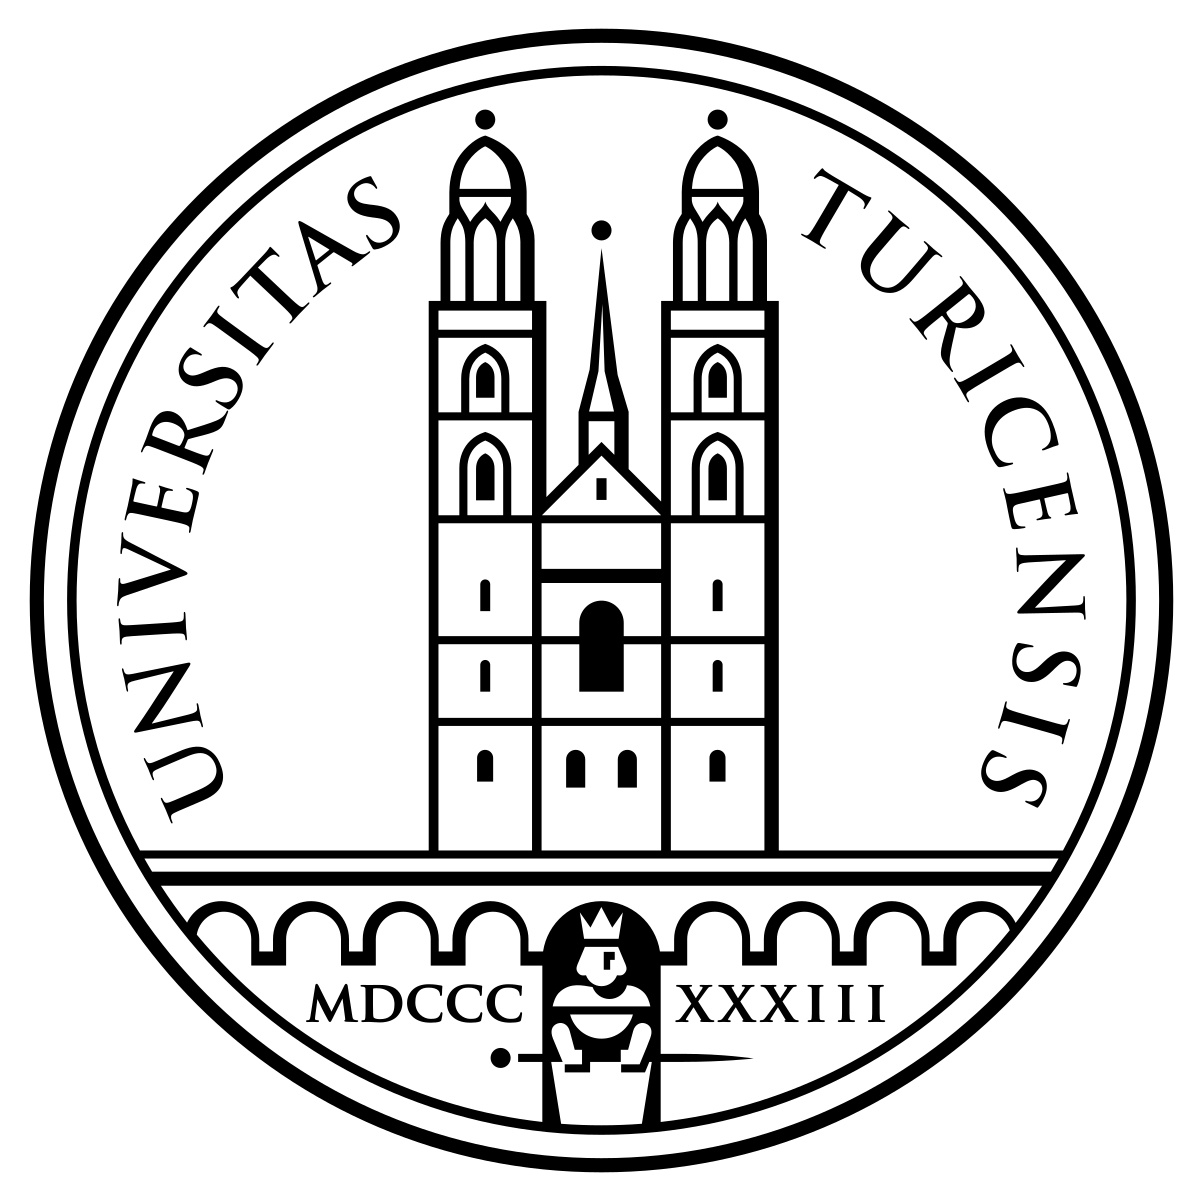
\includegraphics[width=0.4\textwidth]{../../figures/University_of_Zurich_seal.png} % Add your project logo
    
    \vspace{2cm}
    \Huge
    \textbf{Analysis of Deposit Rate Pass Through Effects in Tightening Cycles}
    
    \vspace{1cm}
    \LARGE
    This research project focuses on examining how savings deposit rates within Switzerland respond to changes in central bank policy rates. 
    
    \vspace{1cm}
    \textbf{Authors:}\\ John Hojnacki \\ Matthew Aylward \\ Victoria Gemperle
    \vspace{1cm}
    
    \textbf{Date:}\\
    \thedate
    \vfill
    
\end{titlepage}

\section{Introduction}

\linespread{1}  % Adjust the factor as needed

Central banks globally employ a variety of methods to implement monetary policy, with a key mechanism often being the short-term policy rate. This rate influences the borrowing costs of commercial banks from the central bank, setting a baseline for other interest rates in the economy. Understanding how other rates, such as consumer deposit rates, respond to changes in the policy rate is crucial for gauging the speed and effectiveness of monetary policy transmission.\\

In this study, we aim to assess the responsiveness of deposit rates on consumer savings accounts to shifts in central bank policy rates across different economic cycles. Deposit rates are particularly significant as they directly impact a large portion of the population. For instance, a 2022 US Consumer Finance Survey revealed that 98.6\% of households possess a transaction account, in contrast to only 11.5\% holding bonds\cite{scf2022}, underscoring the widespread influence of deposit rates.\\

We adopt the concept of the cumulative deposit beta to measure the relative change in deposit rates vis-à-vis policy rates during a rate hiking cycle. This approach, previously applied by researchers at the New York Federal Reserve in a US context\cite{deposit2023}, will be adapted and applied to the Swiss banking sector, with necessary modifications to suit data availability.

\section{Data}

For this analysis, we require monthly data on policy rates and deposit rates. In cases where a specific policy rate target isn't defined, an average value within a target range can be used. Our study focuses on Switzerland, where we utilize data from the Swiss National Bank spanning from 2000 to 2019 based on a target range, and subsequently, a specific target post-2019.\\

Historical availability and consistency of deposit rate data can pose challenges. For instance, a single deposit rate is hard to come by in the US. Researchers at the NY Fed calculate the rate as a ratio of interest paid on deposits to interest-bearing deposits\cite{deposit2023}. We adopted a different approach for Switzerland, using a savings deposit rate available directly from the Swiss National Bank. The choice and treatment of data in this study are guided by the need to represent economically meaningful rates. For future applications of this methodology to different contexts, creativity is encouraged, especially in cases where direct data may not be available or may require adjustment for consistency and comparability.\\

\section{Methodology}

\subsection{Identification of Hiking Cycles}

We derive our own methodology for identifying hiking cycles, utilizing a precise algorithm, with time (\( t \)) measured in monthly intervals. A hiking period is defined as a sequence of months during which there is a consistent increase in the policy rate. The criteria for a month to be considered part of a hiking period are as follows:

\begin{enumerate}
    \item \textbf{Direct Increase:} There must be an observed increase in the policy rate compared to the preceding month.
    
    \item \textbf{Look-Ahead Logic:} A month may also be considered part of a hiking period under the following condition:
    \begin{itemize}
        \item In cases where there is no month-over-month increase in the current period, but there was an increase in the previous period, and an increase is anticipated in the subsequent two months.
    \end{itemize}
\end{enumerate}

This forward-looking approach, termed 'look-ahead logic', is applicable in an ex-post analysis of historical data. The objective is not to predict future rate hikes but to classify them accurately within our dataset. By incorporating both immediate and anticipated policy rate movements, this methodology allows for a comprehensive and accurate identification of hiking periods.\\

\textbf{Inclusion Criteria and Unique Identifiers}

Critical to our analysis is the inclusion of the month preceding an official rate hike. Its inclusion is relevant to anchor the starting point and provide a basis for comparison as the hiking cycle progresses. Furthermore, each identified hiking period is assigned a unique identifier. This facilitates a granular analysis, allowing for a comparative assessment across different cycles.

\subsection{Labeling periods of Rising Deposit Rates}
Once a hiking cycle has commenced, we begin monitoring changes in the deposit rate. This monitoring continues even once the hiking cycle itself has technically ended. The objective is to capture the peak in deposit rates intra-cycle with the logic that capturing changes in deposit rates during the hiking cycle alone would miss the lagged effect of monetary policy pass-through to the economy.

\subsection{Calculation of Deposit Betas}

The deposit beta, (\( \beta_t \)), measures the magnitude of change in deposit rates relative to the change in policy rates, providing insights into the transmission mechanism of monetary policy.\\

The formula used for estimating deposit beta is:
\[
\beta_t = \frac{\Delta D_t}{\Delta P_t}
\]
where \( \Delta D_t \) represents the total change in deposit rates, and \( \Delta P_t \) denotes the total change in policy rates over the same period. The variable \( t \) signifies the time in months from the start of the hiking cycle. This calculation enables us to quantify the sensitivity of deposit rates to shifts in monetary policy.\\

\textbf{Interpretation of Results}

A higher value of \( \beta_t \) indicates a more pronounced response of deposit rates to changes in policy rates. By tracking the evolution of deposit beta from the onset of a hiking cycle to the peak of deposit rates, we gain an understanding of the lag and magnitude of the banking sector's response to central bank actions. This analysis is particularly pertinent in assessing the efficiency and impact of monetary policy.\\

The methodology applied in this project is designed to be replicable across different countries and time periods, which allows for its usage in scenarios where central banks provide explicit targets, target ranges, or operate without a clearly defined target. The project can be employed to analyze and compare the sensitivity of deposit rates on consumer savings accounts to changes in central banks’ policy rates across different economic and temporal contexts. This cross-country and cross-temporal applicability assures the project's utility in capturing variations in monetary policy transmission mechanisms globally.\\

\section{Applied Analysis: Switzerland}

We now turn to Switzerland with the methodology to a) identify hiking cycles, and b) measure the deposit beta throughout these identified cycles.\\

\subsection{History in a Swiss Context}

In December of 1999, the Swiss National Bank (‘SNB’) announced its intention to steer money market rates through the mechanism of a target range, marking a significant shift in its monetary policy strategy. This change coincided with the decision to begin tightening monetary policy over the next year \cite{snb1999monetary}, providing a crucial context for our analysis, which begins in January of 2000.

\begin{figure}[h]
    \centering
    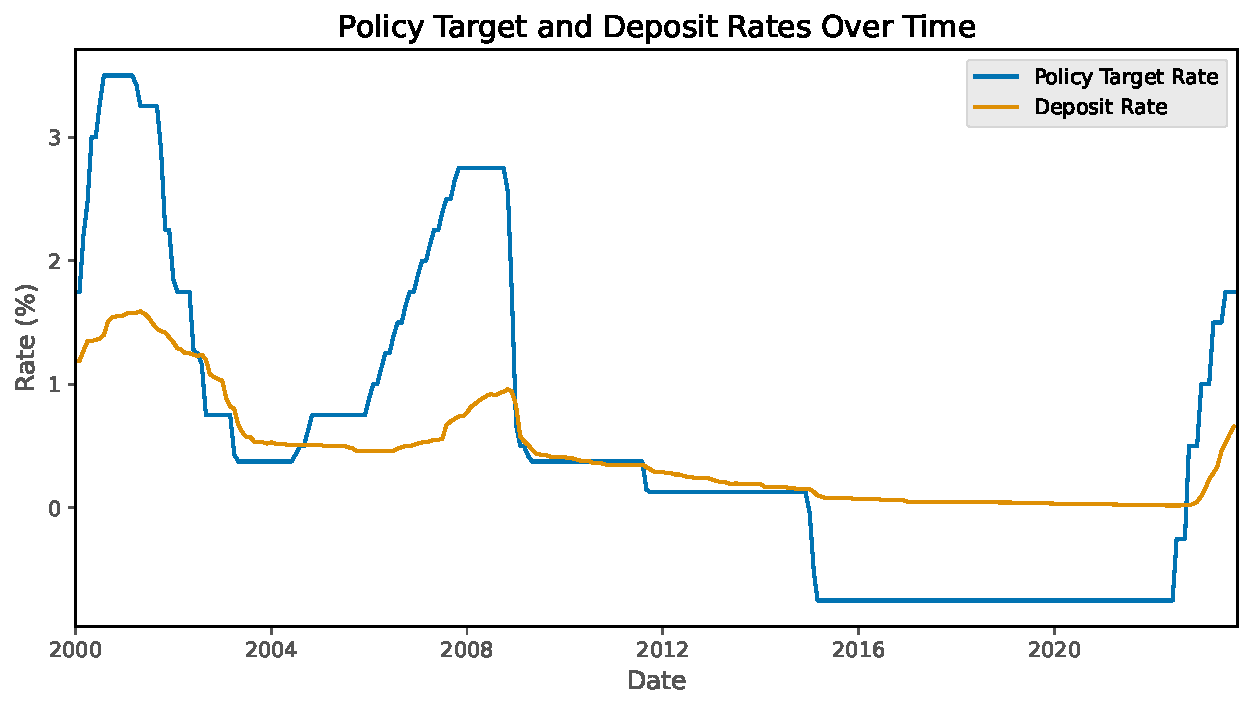
\includegraphics[width=1\textwidth]{../../figures/rates_time_SNB.pdf}
    \caption{Interest rate history for Switzerland, Source: SNB Data Portal\cite{snb2023}}
    \label{fig:rates_time}
\end{figure}

Figure \ref{fig:rates_time} presents a comprehensive view of the interest rate history in Switzerland. The graph highlights significant shifts in policy rates and provides an initial visual representation of how these rates have fluctuated over time. 

\subsection{Identification of Hiking Cycles}

\begin{figure}[h!]
    \centering
    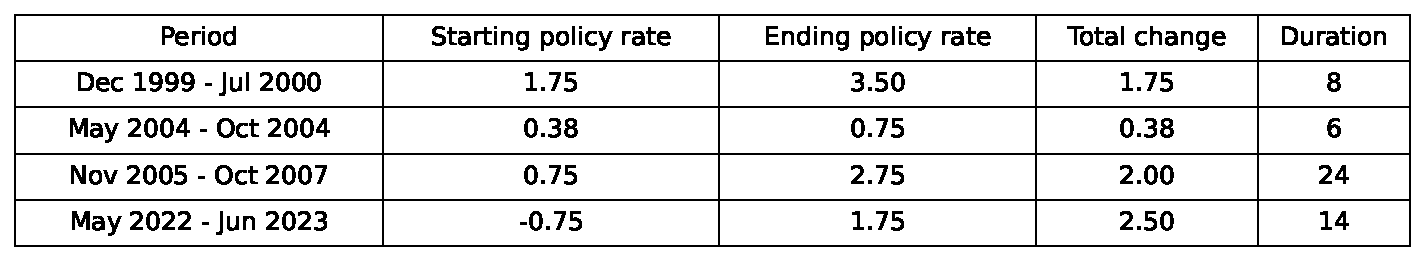
\includegraphics[width=1\textwidth]{../../figures/hiking_summary_SNB.pdf}
    \caption{Hiking Cycles Across Time, Source: SNB Data Portal\cite{snb2023}, Own calculations}
    \label{fig:hiking_cycles}
\end{figure}

Figure \ref{fig:hiking_cycles} delineates the identified hiking cycles in Switzerland. Our analysis reveals four distinct periods of policy rate increases: 2000, 2004, 4Q05-, and 2022-2023. This graph not only illustrates the duration but also the intensity of each hiking cycle.\\

\textbf{2000 Hiking Cycle}: The first cycle in our analysis period marked a significant phase of monetary tightening, as the SNB began to shift its policy stance in response to changing economic conditions at the turn of the millennium.\\

\textbf{2004 Hiking Cycle}: Although the 2004 cycle technically qualifies as a rate hike, we exclude it from our detailed analysis. This brief period was not a true tightening of monetary conditions but rather a reversal of the cuts made in 2003 to counter deflationary trends, as indicated by the SNB's monetary policy report\cite{snb2004monetary}. Our focus remains on more substantial policy shifts.\\

\textbf{4Q05- Hiking Cycle}: This period, beginning in the fourth quarter of 2005, represented another phase of policy tightening. The changes in this cycle were more gradual, reflecting the SNB's adaptive approach to evolving economic indicators and conditions.\\

\textbf{2022-2023 Hiking Cycle}: The most recent cycle in our analysis, this period is particularly noteworthy due to its context within the post-Covid-19 economic recovery. The SNB's policy adjustments during this time are critical for understanding the current dynamics of monetary policy transmission in Switzerland.\\

By examining these cycles, especially the more economically significant ones, our analysis aims to provide a nuanced understanding of the relationship between policy rate changes and their effects on consumer financial products.\\

\begin{figure}[h!]
    \centering
    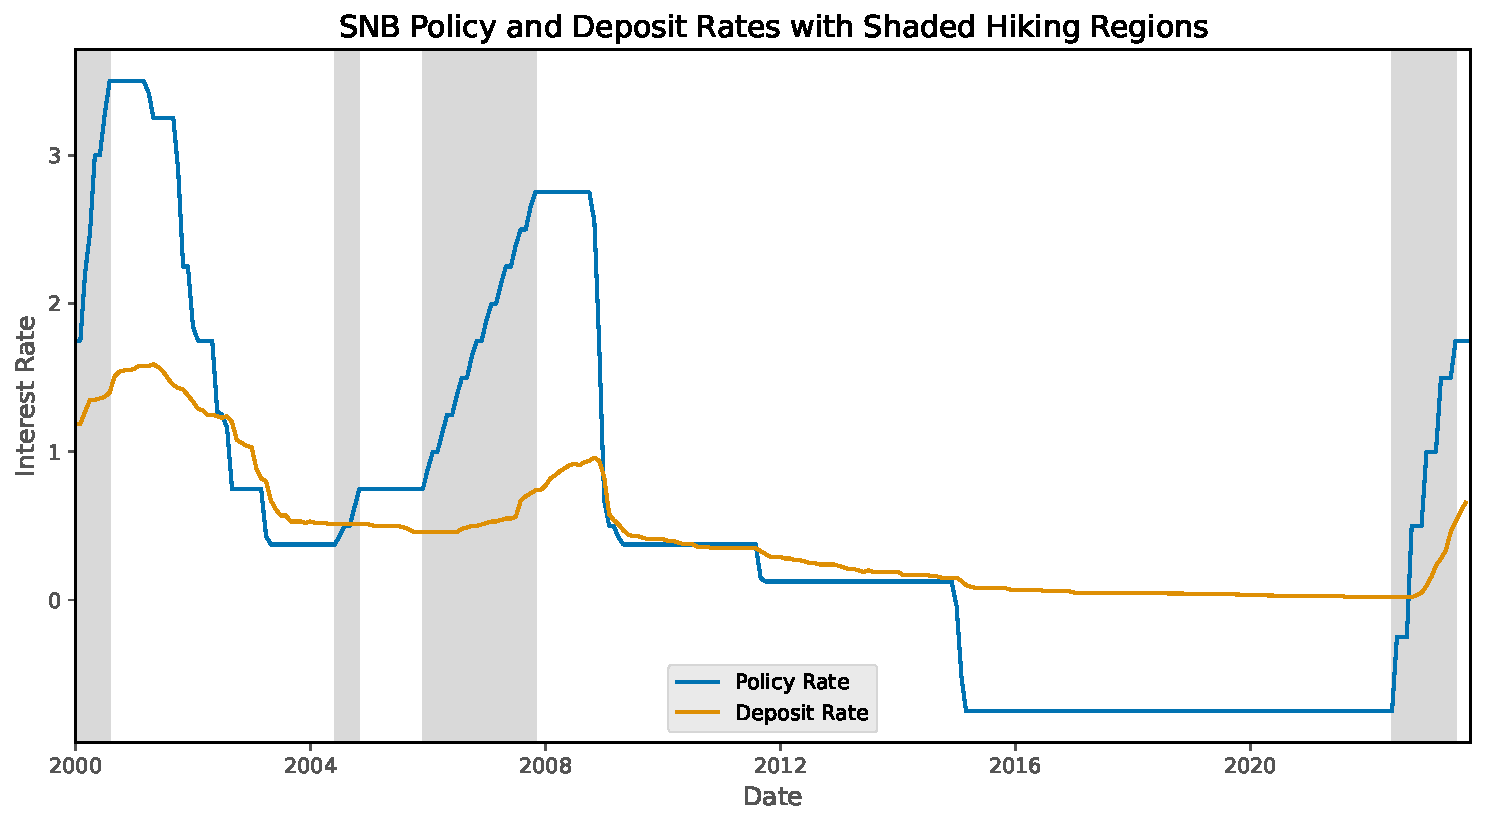
\includegraphics[width=1\textwidth]{../../figures/rates_shaded_SNB.pdf}
    \caption{Interest rate history for Switzerland with shaded regions for hiking cycles, Source: SNB Data Portal\cite{snb2023}, Own calculations}
    \label{fig:rates_shaded}
\end{figure}

\subsection{Labeling Periods of Rising Deposit Rates}

The subsequent analysis of deposit rates during these identified hiking cycles reveals patterns that are crucial for understanding the transmission of policy changes to consumer financial products.

\begin{figure}[h!]
    \centering
    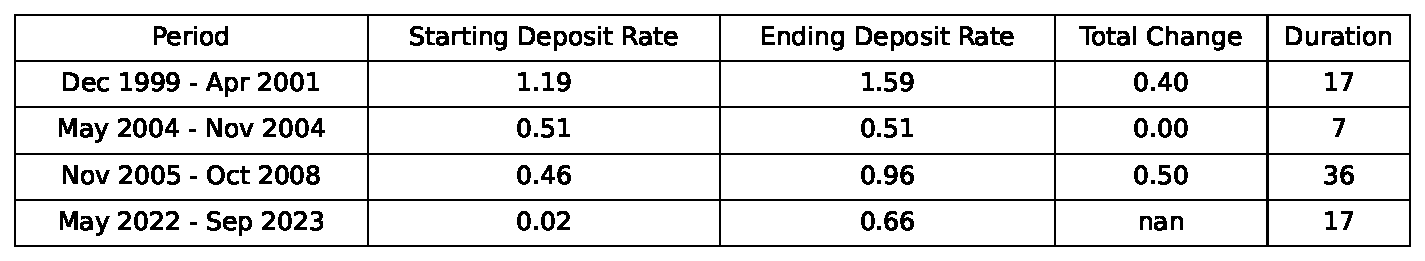
\includegraphics[width=1\textwidth]{../../figures/deposit_summary_SNB.pdf}
    \caption{Deposit Rates Summary across Hiking Periods, Source: SNB Data Portal\cite{snb2023}, Own calculations}
    \label{fig:deposit_summary}
\end{figure}

Figure \ref{fig:deposit_summary} shows how deposit rates responded during and after the identified hiking periods. The lag in response and the peak of deposit rates provide insights into the banking sector's reaction to policy changes. This figure is particularly informative when considering the different economic contexts of each hiking cycle.

\subsection{Calculation of Deposit Betas}

In line with our earlier methodology, we calculated deposit betas for each identified hiking cycle in Switzerland. This metric is particularly useful for comparing cycles that vary in their starting points and lengths, where absolute or simple relative changes in rates might not provide a complete picture.

\begin{figure}[h!]
    \centering
    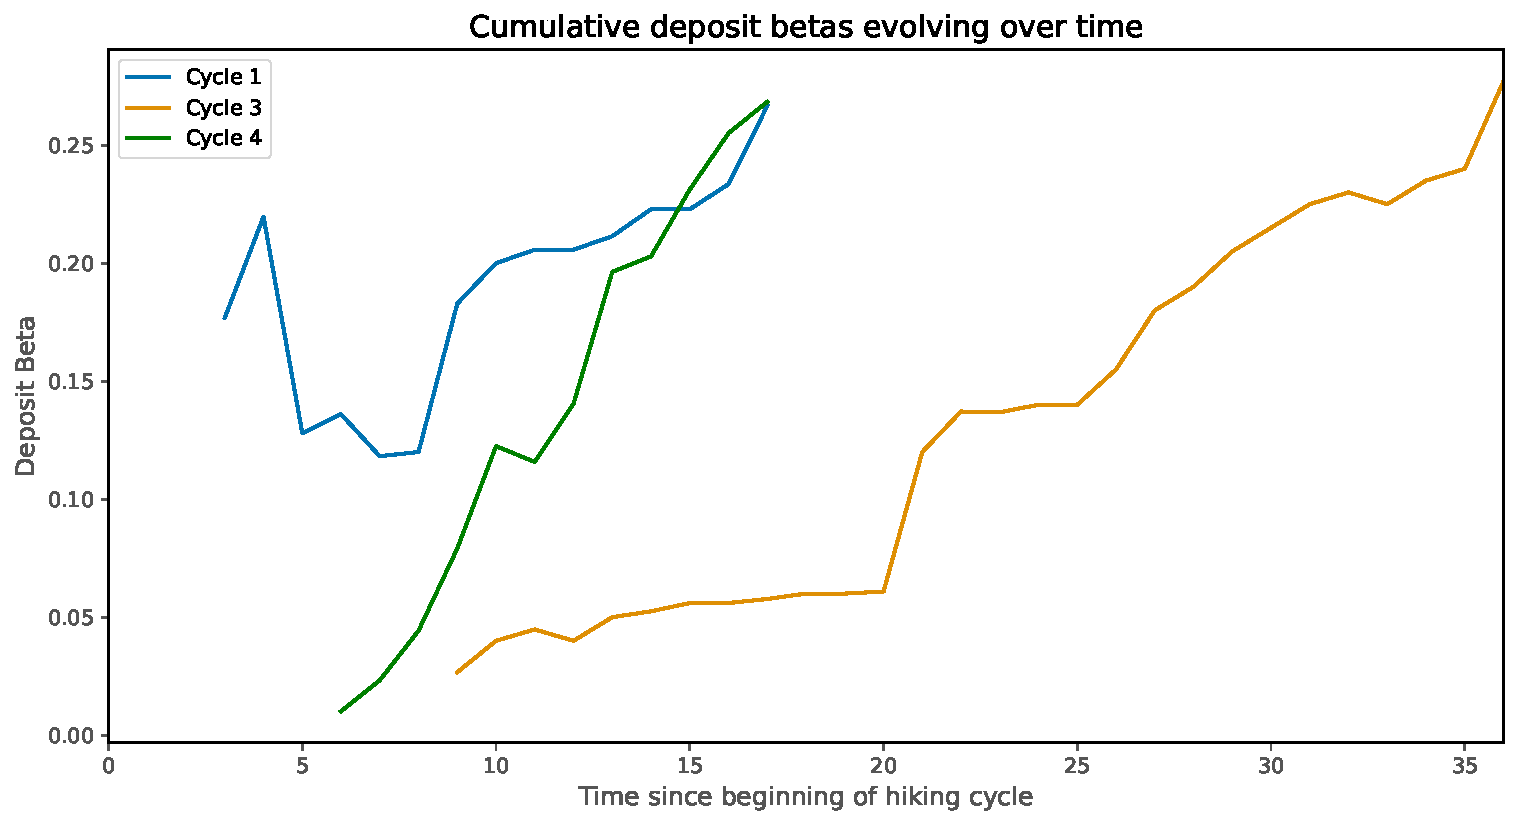
\includegraphics[width=1\textwidth]{../../figures/deposit_beta_SNB.pdf}
    \caption{Cumulative Swiss Deposit Betas in Hiking Cycles, Source: SNB Data Portal\cite{snb2023}, Own calculations}
    \label{fig:deposit_betas}
\end{figure}

Figure \ref{fig:deposit_betas} displays the cumulative Swiss Deposit Betas for the various hiking cycles. The graphical representation allows for a nuanced comparison of how deposit rate sensitivity to policy rate changes has evolved over distinct economic periods. This is especially critical when analyzing cycles that begin from different policy rate levels or have varying durations. By normalizing the changes in deposit rates relative to policy rates, deposit betas provide a more standardized and comparable measure across different monetary policy environments. This analytical approach offers a deeper understanding of the transmission of monetary policy in Switzerland.

\subsection{Discussion of Results}

The analysis of deposit rate responses to monetary policy changes in Switzerland reveals complex dynamics, particularly when comparing the current tightening cycle with previous periods such as the 2000 hikes. A key observation is that while the total pass-through of policy rate changes to deposit rates appears similar approximately five months into both cycles, the underlying factors and timelines differ significantly.\\

In the current cycle, policy rates began below zero, a unique starting point that influenced the initial response of deposit rates. For about the first six months, there was minimal pressure on deposit rates to adjust, likely due to the negative starting point of policy rates. However, once adjustments began, the deposit rates responded more rapidly than in previous cycles. This indicates that the magnitude of response in the current cycle might be understated if one only considers the total pass-through percentage without accounting for the delayed start.\\

The comparison with the 2000 hikes underscores this point. In that cycle, deposit rates took longer to start moving, but eventually achieved a comparable level of pass-through. The quicker response in the current cycle, despite the delayed start, suggests a banking sector that is now more sensitive to policy changes, potentially reflecting a shift in market dynamics or monetary policy strategy.\\

This analysis, however, must be contextualized within its limitations. The focus on Swiss data may not fully capture global banking trends, and external factors such as international economic conditions are not considered in this study. Nonetheless, these findings provide valuable insights into the evolving relationship between central bank policy rates and the banking sector's response, highlighting the need for a nuanced understanding of monetary policy transmission in different economic contexts.\\

\section{Conclusion}

This study has provided an examination of the response of deposit rates to policy rate changes in Switzerland. The findings reveal a notable change in the banking sector's responsiveness to monetary policy, particularly in the current tightening cycle. The higher and faster pass-through of policy rate changes to deposit rates underscores a more dynamic interplay between central bank actions and the banking sector.\\

These insights are crucial for understanding the effectiveness of monetary policy as a tool for economic management. They also have significant implications for savers and borrowers, affecting the financial decisions of households and businesses.\\

Future research could expand this analysis to other countries and economic cycles, enhancing our understanding of the global dynamics of monetary policy transmission. Additionally, investigating the role of other economic factors and their interaction with central bank policies would provide a more holistic view of the financial ecosystem.\\

% Bibliography section
\newpage  % Start a new page for the bibliography
\section{References}
\printbibliography[heading=none] 

\end{document}